% !TEX root = ../Hamiltonian_of_mean_force.tex
\section{Branch-Resolved Tilt-Angle Continuation for the Qubit Mean-Force State (Standalone Appendix Draft)}
\label{app:branch_alignment_codex}

This standalone appendix draft records a sign-resolved derivation of the qubit
geometry underlying the apparent ``reflection'' in
Fig.~\ref{fig:bloch_disk_portrait}(b).  The central point is that the branch
ambiguity lives in the \emph{tilt-angle chart} (principal inverse tangent),
whereas the Cartesian Bloch vector remains continuous.  When the tilt angle is
continued across the principal-branch cut in the correct way, the trajectory is
interpreted as a continuous precession toward the coupling direction
$\hat{\mathbf f}$ rather than a physical reflection at the chart image
$\pi-\alpha_f$.

\subsection{The influence operator in the same rapidity form as $\rho_Q$}

The cleanest way to locate the origin of the large angle $\Theta$ is to first
write the \emph{symmetrized influence operator} in the same matrix form as the
final reduced state.  Starting from Appendix~\ref{app:qubit_ladder_derivation},
\begin{equation}
    S = \Delta_0 \mathbb{I} + \Delta_z \sigma_z
      + \Delta_\perp \bigl(\sigma_x\cos\phi_f + \sigma_y\sin\phi_f\bigr),
    \label{eq:branch_codex_S_def}
\end{equation}
define its traceless part
\begin{equation}
    M \equiv S-\Delta_0\mathbb{I},
    \qquad
    M^2=\chi^2\mathbb{I},
    \qquad
    \chi = \sqrt{\Delta_z^2+\Delta_\perp^2}.
\end{equation}
The exact exponential is then
\begin{equation}
    e^S = e^{\Delta_0}\cosh\chi\left(\mathbb{I} + \gamma M\right),
    \qquad
    \gamma \equiv \frac{\tanh\chi}{\chi}.
    \label{eq:branch_codex_expS}
\end{equation}

It is therefore natural to define the \emph{normalized influence state}
\begin{equation}
    \rho_{\Delta} \equiv \frac{e^S}{\Tr e^S}
    = \frac{1}{2}\left(\mathbb{I} + \gamma M\right),
    \label{eq:branch_codex_rhoDelta}
\end{equation}
which is the density matrix associated with the influence operator alone,
before recombination with the bare Gibbs factor.

Writing
\begin{equation}
    u \equiv \gamma \Delta_z,
    \qquad
    q \equiv \gamma \Delta_\perp,
\end{equation}
we obtain in the qubit energy basis
\begin{equation}
    \rho_{\Delta}
    = \frac{1}{2}
    \begin{pmatrix}
        1+u & q\,e^{-i\phi_f}\\
        q\,e^{+i\phi_f} & 1-u
    \end{pmatrix},
    \qquad
    u^2+q^2 = \tanh^2\chi.
    \label{eq:branch_codex_rhoDelta_matrix}
\end{equation}

\paragraph{Influence rapidity $\theta_\Delta$.}
Introduce the longitudinal influence rapidity
\begin{equation}
    \theta_\Delta \equiv \operatorname{arctanh}(u),
    \label{eq:branch_codex_thetaDelta}
\end{equation}
so that $1\pm u = e^{\pm\theta_\Delta}/\cosh\theta_\Delta$.  Defining
\begin{equation}
    \kappa \equiv q \cosh\theta_\Delta
    = \frac{q}{\sqrt{1-u^2}},
    \label{eq:branch_codex_kappa_from_q}
\end{equation}
the influence-only density takes the same ``angular'' form as $\rho_Q$:
\begin{equation}
    \rho_{\Delta}
    = \frac{1}{2}
    \begin{pmatrix}
        1+\tanh\theta_\Delta &
        \kappa\,\operatorname{sech}\theta_\Delta\,e^{-i\phi_f}\\
        \kappa\,\operatorname{sech}\theta_\Delta\,e^{+i\phi_f} &
        1-\tanh\theta_\Delta
    \end{pmatrix}.
    \label{eq:branch_codex_rhoDelta_angular}
\end{equation}
This is the direct precursor of the final reduced-state expression.

\paragraph{Origin of the manuscript's large angle $\Theta$.}
The reduced state is obtained by recombining the influence exponential with the
bare Gibbs factor.  In the energy basis the bare factor contributes the
diagonal rapidity
\begin{equation}
    a \equiv \frac{\beta\omega_q}{2},
\end{equation}
so the diagonal weights pick up factors $e^{\mp a}$.  Comparing diagonal matrix
elements shows immediately that the final longitudinal rapidity is \emph{not} a
new angle but a shifted influence rapidity:
\begin{equation}
    \Theta = \theta_\Delta - a
    = \operatorname{arctanh}(u)-a.
    \label{eq:branch_codex_bigTheta_origin}
\end{equation}
Thus the large angle $\Theta$ is the recombined longitudinal rapidity after the
bare Gibbs and influence rapidities are merged.

\paragraph{Where the branch issue can appear.}
On the real exact solution, $\operatorname{arctanh}(u)$ is not the periodic
branch source.  The branch ambiguity enters later, when the \emph{tilt angle}
$\varphi$ is extracted from its tangent (Eq.~\eqref{eq:branch_codex_tanphi}
below).  The relevant singular chart is therefore the tilt-angle chart, not the
fixed mixing angle $\theta$.

\subsection{Clean branch analysis in the rewritten \texorpdfstring{$(\chi,\eta,\Theta)$}{(chi,eta,Theta)} variables}

For the branch question, the rewritten `05\_results\_v2.tex' form is the
shortest route.  The exact Bloch components satisfy
\begin{equation}
    \begin{split}
        m_z &= \tanh\Theta,\\
        m_\perp &= \tan\eta\left(m_z\cosh a + \sinh a\right),
    \end{split}
    \qquad a \equiv \frac{\beta\omega_q}{2},
    \label{eq:branch_codex_bloch_locking_linear}
\end{equation}
with
\begin{equation}
    \Theta = \operatorname{arctanh}(u)-a,
    \qquad
    \tan\eta = -\cot\theta\,\frac{\Sigma_\perp}{\Sigma_z}.
    \label{eq:branch_codex_theta_eta_params}
\end{equation}
The purity is still
\begin{equation}
    r = \sqrt{m_z^2+m_\perp^2} = \tanh\chi.
    \label{eq:branch_codex_purity_rewritten}
\end{equation}

\paragraph{Why this is the right separation.}
This form cleanly separates:
\begin{itemize}
    \item \textbf{radius/crossover:} controlled by $\chi$ through $r=\tanh\chi$;
    \item \textbf{orientation geometry:} controlled by $(\Theta,\eta)$;
    \item \textbf{mixing-angle dependence:} carried explicitly by
    $\tan\eta \propto \cot\theta$.
\end{itemize}
The branch issue is therefore an \emph{angle-chart} issue on top of a
$\chi$-controlled crossover.

\paragraph{Influence polar angle and the exact \texorpdfstring{$u(\chi)$}{u(chi)} identity.}
Introduce the polar decomposition of the symmetrized influence vector
\begin{equation}
    \Delta_z = \chi\cos\eta,
    \qquad
    \Delta_\perp = \chi\sin\eta,
    \label{eq:branch_codex_delta_polar}
\end{equation}
so that $\tan\eta=\Delta_\perp/\Delta_z$ agrees with
Eq.~\eqref{eq:branch_codex_theta_eta_params}.  Since
\begin{equation}
    u = \gamma\Delta_z,
    \qquad \gamma = \frac{\tanh\chi}{\chi},
\end{equation}
we obtain the exact identity
\begin{equation}
    u = \cos\eta\,\tanh\chi.
    \label{eq:branch_codex_u_chi_eta}
\end{equation}
Hence the longitudinal rapidity becomes a direct function of $\chi$:
\begin{equation}
    \Theta(\chi)
    = \operatorname{arctanh}\!\bigl(\cos\eta\,\tanh\chi\bigr)-a.
    \label{eq:branch_codex_Theta_of_chi}
\end{equation}

\paragraph{Branch scale in \texorpdfstring{$\chi$}{chi}.}
The tilt-angle chart singularity occurs at $\Theta=0$ (equivalently $m_z=0$),
so the branch locus is
\begin{equation}
    \Theta(\chi_b)=0
    \quad\Longleftrightarrow\quad
    \cos\eta\,\tanh\chi_b = \tanh a.
    \label{eq:branch_codex_branch_scale_condition}
\end{equation}
When a solution exists, this defines a branch scale
\begin{equation}
    \chi_b = \operatorname{arctanh}\!\left(\frac{\tanh a}{\cos\eta}\right).
    \label{eq:branch_codex_chi_b}
\end{equation}
This is the clean way to compare the branch event to the crossover scale
$\chi=1$.

\paragraph{Equivalence to the older \texorpdfstring{$(u,\kappa)$}{(u,kappa)} variables.}
For cross-checking signs and matrix elements one may still use
\begin{equation}
    \tan\eta
    = \frac{\Delta_\perp}{\Delta_z}
    = \frac{q}{u},
    \qquad
    \kappa
    = \frac{q}{\sqrt{1-u^2}}
    = \tan\eta\,\sinh\theta_\Delta.
    \label{eq:branch_codex_kappa_eta_thetaDelta}
\end{equation}
These are exact rewritings, not new assumptions.

\subsection{Signed Bloch components from the exact qubit formulas (sign-check form)}

The exact qubit state in Sec.~\ref{subsec:qubit_exact_geometry} is written as
\begin{equation}
    \rho_Q = \frac{1}{2}
    \begin{pmatrix}
        1+\tanh\Theta & \kappa \,\operatorname{sech}\Theta\,e^{-i\phi_f}\\
        \kappa \,\operatorname{sech}\Theta\,e^{+i\phi_f} & 1-\tanh\Theta
    \end{pmatrix},
\end{equation}
with
\begin{equation}
    \Theta = \operatorname{arctanh}(u)-a,
    \qquad
    u \equiv \gamma \Delta_z = \gamma s^2\Sigma_z,
    \qquad
    a \equiv \frac{\beta\omega_q}{2},
\end{equation}
and
\begin{equation}
    \kappa = \frac{q}{\sqrt{1-u^2}}
    = \frac{-\gamma c s \Sigma_\perp}{\sqrt{1-u^2}}.
\end{equation}

The main text often uses the magnitude
$r_\perp = |\kappa\operatorname{sech}\Theta|$, which is appropriate for purity
and radial geometry but erases the transverse sign.  For branch diagnostics we
instead define the signed transverse component in the coupling plane:
\begin{equation}
    m_\perp^{(\mathrm{signed})} \equiv \kappa\operatorname{sech}\Theta,
    \qquad
    m_z \equiv \tanh\Theta .
\end{equation}

\paragraph{Rational form of the longitudinal component.}
Using $\tanh(x-y)=\frac{\tanh x-\tanh y}{1-\tanh x\,\tanh y}$ and
$\tanh(\operatorname{arctanh}u)=u$ gives
\begin{equation}
    m_z = \tanh\Theta
    = \frac{u-\tanh a}{1-u\tanh a}.
    \label{eq:branch_codex_mz_rational}
\end{equation}

\paragraph{Rational form of the signed transverse component.}
Using
\begin{equation}
    \cosh(\operatorname{arctanh}u-a)
    = \frac{\cosh a - u \sinh a}{\sqrt{1-u^2}},
\end{equation}
we obtain
\begin{equation}
    \operatorname{sech}\Theta
    = \frac{\sqrt{1-u^2}}{\cosh a - u \sinh a},
\end{equation}
and therefore
\begin{equation}
    m_\perp^{(\mathrm{signed})}
    = \frac{-\gamma c s \Sigma_\perp}{\cosh a - u \sinh a}.
    \label{eq:branch_codex_mperp_rational}
\end{equation}

This form makes the sign structure explicit: the numerator carries the sign of
$-\Sigma_\perp$, while the denominator is positive for finite $a$ and $|u|<1$,
since
\begin{equation}
    \cosh a - u\sinh a
    = \cosh a\,\bigl(1-u\tanh a\bigr) > 0.
    \label{eq:branch_codex_positive_denom}
\end{equation}
Hence any apparent reflection in the plotted trajectory cannot come from a
physical pole in the exact state.  These rational forms are best read as
\emph{sign-check formulas} complementing the more transparent angular locking
form in Eq.~\eqref{eq:branch_codex_bloch_locking_linear}.

\subsection{Explicit derivation of $\mathbf h_{\rm eff}$ from the symmetrized exponent}

Appendix~\ref{app:qubit_ladder_derivation} gives the symmetrized operator
\begin{equation}
    S = \Delta_0 \mathbb{I} + \Delta_z \sigma_z
      + \Delta_\perp\bigl(\sigma_x\cos\phi_f + \sigma_y\sin\phi_f\bigr).
\end{equation}
For geometric analysis in the coupling plane we define $\hat{\mathbf n}_s$ as
the bare system axis and $\hat{\mathbf e}_{\perp}^{(s)}$ as the unit vector in
the coupling plane orthogonal to $\hat{\mathbf n}_s$ and pointing along the
transverse projection of $\hat{\mathbf f}$, so that
\begin{equation}
    \hat{\mathbf f} = s\,\hat{\mathbf e}_{\perp}^{(s)} + c\,\hat{\mathbf n}_s.
\end{equation}
The traceless part of $S$ defines the effective influence vector
\begin{equation}
    \mathbf h_{\rm eff}
    \equiv \Delta_\perp\,\hat{\mathbf e}_{\perp}^{(s)}
         + \Delta_z\,\hat{\mathbf n}_s,
    \label{eq:branch_codex_heff_energy_basis}
\end{equation}
with the exact coefficients
\begin{equation}
    \Delta_\perp = -c s \Sigma_\perp,
    \qquad
    \Delta_z = s^2 \Sigma_z .
    \label{eq:branch_codex_delta_components}
\end{equation}

\subsection{Coupling-adapted decomposition and orthogonality condition}

Define the unit vector in the coupling plane orthogonal to $\hat{\mathbf f}$:
\begin{equation}
    \hat{\mathbf n}^{(f)}_\perp
    \equiv \frac{\hat{\mathbf n}_s - c\hat{\mathbf f}}{s}
    = -c\,\hat{\mathbf e}_{\perp}^{(s)} + s\,\hat{\mathbf n}_s.
\end{equation}
Because $\{\hat{\mathbf f},\hat{\mathbf n}^{(f)}_\perp\}$ is orthonormal, the
coefficients are simply scalar projections:
\begin{equation}
    \mathbf h_{\rm eff} = A_f \hat{\mathbf f} + A_\perp \hat{\mathbf n}^{(f)}_\perp,
\end{equation}
with
\begin{align}
    A_f &= \mathbf h_{\rm eff}\cdot\hat{\mathbf f}
        = s\Delta_\perp + c\Delta_z
        = c s^2 (\Sigma_z - \Sigma_\perp),
        \label{eq:branch_codex_Af}\\
    A_\perp &= \mathbf h_{\rm eff}\cdot\hat{\mathbf n}^{(f)}_\perp
        = -c\Delta_\perp + s\Delta_z
        = s\bigl(c^2\Sigma_\perp + s^2\Sigma_z\bigr).
        \label{eq:branch_codex_Aperp}
\end{align}

\paragraph{Orthogonality hypothesis.}
The condition for $\mathbf h_{\rm eff}$ to be exactly orthogonal to
$\hat{\mathbf f}$ is
\begin{equation}
    A_f = 0
    \quad\Longleftrightarrow\quad
    \Sigma_z = \Sigma_\perp
    \qquad (c\neq 0,\ s\neq 0).
    \label{eq:branch_codex_heff_orthogonal_condition}
\end{equation}
This is a specific channel-balance condition, not a generic identity.

\paragraph{Consistency check against the current Sec.~6 draft.}
The present derivation yields
$A_\perp = s(c^2\Sigma_\perp + s^2\Sigma_z)$
[Eq.~\eqref{eq:branch_codex_Aperp}].  The current Sec.~6 draft
(``physical\_regimes\_v2'') writes the $\hat{\mathbf n}_\perp^{(f)}$ coefficient
as $s(\Sigma_\perp c + \Sigma_z s^2)$.  If the same basis and channel
definitions are intended, this appears to differ by one factor of $c$ in the
non-resonant term.  This note flags the discrepancy only; no manuscript change
is made here.

\subsection{Tilt-angle branch crossing and continuation (the clean version)}

The branch lives in the \emph{tilt angle} $\varphi$ chart, not in the fixed
mixing angle $\theta$.  In the rewritten variables the exact tilt angle
satisfies
\begin{equation}
    \tan\varphi
    = -\frac{m_\perp}{m_z}
    = -\tan\eta\left(\cosh a + \sinh a\,\coth\Theta\right),
    \qquad a\equiv \frac{\beta\omega_q}{2},
    \label{eq:branch_codex_tanphi}
\end{equation}
which is equivalent to $\tan\varphi=-\kappa/\sinh\Theta$ but makes the two
roles transparent: $\eta$ sets the geometric prefactor, while $\Theta$ carries
the chart singularity through $\coth\Theta$.

\paragraph{Direct dependence on the mixing angle \texorpdfstring{$\theta$}{theta}.}
Substituting the exact influence-ratio definition
$\tan\eta=-\cot\theta\,(\Sigma_\perp/\Sigma_z)$ from
Eq.~\eqref{eq:branch_codex_theta_eta_params} directly into
Eq.~\eqref{eq:branch_codex_tanphi} gives
\begin{equation}
    \tan\varphi
    =
    \cot\theta\,\frac{\Sigma_\perp}{\Sigma_z}
    \left(\cosh a + \sinh a\,\coth\Theta\right),
    \qquad a=\frac{\beta\omega_q}{2}.
    \label{eq:branch_codex_tanphi_expanded_theta}
\end{equation}
This is the explicit form in which the dependence of the \emph{tilt angle}
on the \emph{mixing angle} is visible at a glance.

\paragraph{Temperature-dependent sign of the transverse/longitudinal ratio.}
Equation~\eqref{eq:branch_codex_tanphi_expanded_theta} also makes clear that
the sign of the tilt-angle chart variable is controlled by the product
\begin{equation}
    X
    =
    \cot\theta\,
    \frac{\Sigma_\perp}{\Sigma_z}\,
    B(\Theta,a),
    \qquad
    B(\Theta,a)\equiv \cosh a + \sinh a\,\coth\Theta,
    \label{eq:branch_codex_X_sign_factorized}
\end{equation}
so that
\begin{equation}
    \operatorname{sgn}X
    = \operatorname{sgn}(\cot\theta)\,
      \operatorname{sgn}\!\left(\frac{\Sigma_\perp}{\Sigma_z}\right)\,
      \operatorname{sgn}B(\Theta,a).
    \label{eq:branch_codex_sgnX_factorized}
\end{equation}
This isolates a second source of apparent angular ``flips'' besides the
principal-$\arctan$ branch cut: the ratio $\Sigma_\perp/\Sigma_z$ itself can
change sign as a function of temperature.

In the rewritten channel coefficients, the transverse coefficient
$\Sigma_\perp(\beta)$ is a difference of contributions (with different
temperature dependence), so it can pass through zero while $\Sigma_z(\beta)$
retains its sign on the same parameter slice.  When this happens,
\begin{equation}
    \Sigma_\perp(\beta_0)=0
    \quad\Longrightarrow\quad
    \tan\eta(\beta_0)=0
    \quad\Longrightarrow\quad
    m_\perp(\beta_0)=0,
    \label{eq:branch_codex_sigma_perp_zero}
\end{equation}
and for temperatures on opposite sides of $\beta_0$ one has opposite signs of
$\tan\eta$ (equivalently opposite signs of the transverse tilt prefactor in
Eq.~\eqref{eq:branch_codex_tanphi_expanded_theta}).

This is distinct from the branch locus $\Theta=0$: a sign flip of
$\Sigma_\perp/\Sigma_z$ changes the \emph{orientation side} of the tilt angle,
whereas $\Theta=0$ drives the \emph{principal-chart singularity}.  In
particular, the branch scale $\chi_b$ from Eq.~\eqref{eq:branch_codex_chi_b}
depends on $\cos\eta$ and is therefore insensitive to $\eta\to-\eta$ (for a
fixed sign of $\Delta_z$), while the sign of $\tan\eta$ still flips.  This is
an additional reason the angle must be continued by continuity: otherwise a
temperature-driven sign change of $\Sigma_\perp/\Sigma_z$ can be misread as a
geometric reflection rather than a smooth passage through $m_\perp=0$.

Using the trigonometric identity
\begin{equation}
    \cot\theta = \tan\!\left(\frac{\pi}{2}-\theta\right),
    \label{eq:branch_codex_cot_shift_identity}
\end{equation}
one may equivalently read the geometric prefactor as a \emph{$\pi/2$-shifted}
tangent.  This is the clean way to see why the branch-corrected continuation of
the tilt angle can look like a precession ``around'' the apparent reflected
branch in a principal-angle plot.

\paragraph{Explicit vs implicit \texorpdfstring{$\theta$}{theta}-dependence.}
Equation~\eqref{eq:branch_codex_tanphi_expanded_theta} separates two effects:
\begin{enumerate}
    \item \textbf{Explicit geometric factor:}
    \begin{equation}
        \cot\theta,
    \end{equation}
    which directly amplifies/suppresses the tilt as the coupling geometry is
    moved toward longitudinal/transverse alignment.
    \item \textbf{Implicit dressing dependence through $\Theta(\beta,g,\theta)$:}
    \begin{equation}
        \Theta(\beta,g,\theta)
        = \operatorname{arctanh}\!\bigl(u(\beta,g,\theta)\bigr)-a,
        \qquad
        u=\gamma(\chi)s^2\Sigma_z,
    \end{equation}
    with
    \begin{equation}
        \chi
        = g^2 s\sqrt{c^2\Sigma_\perp^2+s^2\Sigma_z^2},
        \qquad c=\cos\theta,\ s=\sin\theta.
    \end{equation}
    Thus $\theta$ also feeds back into the longitudinal rapidity through the
    crossover function $\gamma(\chi)=\tanh\chi/\chi$.
\end{enumerate}

\paragraph{Local singular expansion (tilt-chart branch point).}
Near the branch scale $\chi_b$ (equivalently $\Theta=0$), use
$\coth\Theta = \Theta^{-1} + \Theta/3 + O(\Theta^3)$ to obtain
\begin{equation}
    \tan\varphi
    =
    \cot\theta\,\frac{\Sigma_\perp}{\Sigma_z}
    \left(
        \frac{\sinh a}{\Theta}
        + \cosh a
        + \frac{\sinh a}{3}\Theta
        + O(\Theta^3)
    \right).
    \label{eq:branch_codex_tanphi_local_sing}
\end{equation}
This makes the branch anatomy transparent: the divergence driving the
principal-angle jump comes from the $\Theta^{-1}$ term, while the overall sign
and amplitude of that divergence are modulated by the geometric prefactor
$\cot\theta\,(\Sigma_\perp/\Sigma_z)$.

\paragraph{Take \texorpdfstring{$\arctan$}{arctan}: principal branch plus continuity index.}
Define
\begin{equation}
    X(\chi;\beta,\theta)
    \equiv
    -\tan\eta\left(\cosh a + \sinh a\,\coth\Theta(\chi)\right),
    \label{eq:branch_codex_X_def}
\end{equation}
so that $\tan\varphi = X$.  The principal chart gives
\begin{equation}
    \varphi_{\rm pr} = \arctan X \in \left(-\frac{\pi}{2},\frac{\pi}{2}\right),
\end{equation}
but the continuous physical angle in the coupling plane is
\begin{equation}
    \varphi_{\rm cont} = \arctan X + n(\chi)\pi,
    \qquad n(\chi)\in\mathbb{Z},
    \label{eq:branch_codex_varphi_cont_branch_index}
\end{equation}
where $n(\chi)$ is fixed by continuity (equivalently by angle unwrapping).
At $\chi=\chi_b$, one has $X\to\pm\infty$ and therefore
\begin{equation}
    \varphi_{\rm pr}\to \pm\frac{\pi}{2},
\end{equation}
so the apparent branch ``flip'' is exactly the principal $\arctan$ chart
crossing its boundary.

\paragraph{Fig.~7(b): precession vs the apparent reflected branch.}
Panel~(b) of Fig.~\ref{fig:bloch_disk_portrait} uses the folded horizontal
coordinate $\sqrt{m_x}$, which suppresses transverse sign information.  In this
folded representation, a principal-angle branch crossing can appear as a
reflection toward $\pi-\alpha_f$ (with $\alpha_f$ the coupling-axis direction
in the same chart).  The reason is simple: once the transverse sign is folded
out, the chart no longer distinguishes an angle from its reflected image
$\alpha\mapsto \pi-\alpha$.  The correct continuation is instead
\begin{equation}
    \varphi_{\rm cont} = \varphi_{\rm pr} + n\pi,
\end{equation}
which carries the angle \emph{through} the $\pm\pi/2$ chart boundary and yields
a continuous precession around the Bloch disk.  In that continuation, the
trajectory is read as continuing toward alignment with the coupling direction
$\hat{\mathbf f}$ (modulo the expected sign conventions and any
director-vs-vector identification), rather than physically reflecting at the
principal-chart image $\pi-\alpha_f$.

It is useful to state this in terms of a relative angle to the interaction
axis.  Let
\begin{equation}
    \delta_f \equiv \varphi - \alpha_f .
    \label{eq:branch_codex_deltaf_def}
\end{equation}
In the principal chart one sees
\begin{equation}
    \delta_{f,\rm pr} = \varphi_{\rm pr}-\alpha_f,
\end{equation}
which can jump when $\varphi_{\rm pr}$ hits $\pm \pi/2$.  The continuity-corrected
relative angle is instead
\begin{equation}
    \delta_{f,\rm cont}
    = \varphi_{\rm cont}-\alpha_f
    = \delta_{f,\rm pr} + n\pi,
    \label{eq:branch_codex_deltaf_cont}
\end{equation}
with the same branch index $n(\chi)$ as in
Eq.~\eqref{eq:branch_codex_varphi_cont_branch_index}.  The apparent
``reflection'' at $\pi-\alpha_f$ is therefore the principal-chart image of a
trajectory whose continuous continuation is still precessing in the same sense.
In particular, the correct interpretation of an apparent approach to
$\pi-\alpha_f$ in the folded chart is a branch-resolved continuation of
$\delta_f$ toward
\begin{equation}
    \delta_f \to 0
    \quad (\text{vector angle}),
    \qquad\text{or}\qquad
    \delta_f \to 0 \pmod{\pi}
    \quad (\text{director/axis angle}),
\end{equation}
i.e.\ alignment with $\hat{\mathbf f}$ (or its axis), not a physical bounce
off the interaction axis.

By contrast, the Cartesian state components are smooth.  In terms of the signed
coupling-plane components, a branch-safe orientation angle is obtained from
\begin{equation}
    \phi_{\rm wrap}
    \equiv \operatorname{atan2}\!\left(m_\perp^{(\mathrm{signed})},-m_z\right),
    \qquad
    \phi_{\rm cont} \equiv \operatorname{unwrap}\!\left(\phi_{\rm wrap}\right),
    \label{eq:branch_codex_phi_cont}
\end{equation}
where ``unwrap'' denotes the standard numerical branch-tracking procedure that
adds/subtracts integer multiples of $2\pi$ to enforce continuity.

\paragraph{Branch locus.}
The branch event is controlled by
\begin{equation}
    \Theta=0
    \quad\Longleftrightarrow\quad
    u=\tanh a
    \quad\Longleftrightarrow\quad
    m_z=0,
    \label{eq:branch_codex_locus}
\end{equation}
using Eq.~\eqref{eq:branch_codex_mz_rational}.  Equivalently, this is the
condition $\chi=\chi_b$ from Eq.~\eqref{eq:branch_codex_branch_scale_condition}.
At this locus the principal angle inferred from
Eq.~\eqref{eq:branch_codex_tanphi} can jump branches even though the exact
Bloch vector remains continuous.

\paragraph{What changes and what does not.}
Equation~\eqref{eq:branch_codex_tanphi_expanded_theta} shows the separation
cleanly:
\begin{itemize}
    \item changing the mixing angle $\theta$ changes the \emph{prefactor}
    $\tan\eta$ (and therefore the tilt amplitude/sign),
    \item crossing $\Theta=0$ changes the \emph{chart branch} of the principal
    inverse tangent through the $\coth\Theta$ singularity.
\end{itemize}
This is precisely why the branch discussion should be phrased in terms of the
tilt angle $\varphi$, not as a branch of the mixing angle $\theta$.

\paragraph{Continuity enforcement for the tilt angle.}
If one treats $\varphi$ as a \emph{vector} angle, continuity is imposed by
tracking $\phi_{\rm cont}$ in Eq.~\eqref{eq:branch_codex_phi_cont} (or
equivalently $\varphi_{\rm cont}=\arctan X+n\pi$).  If one instead treats the
orientation as an \emph{axis} (director) where antipodal angles are equivalent
modulo $\pi$, the local continuation across the principal-branch cut is
implemented by the reflected chart
\begin{equation}
    \varphi \;\mapsto\; \pi-\varphi
    \qquad\text{(axis/director continuation)}.
    \label{eq:branch_codex_varphi_reflect}
\end{equation}
This is the relevant reflection operation for the tilt-angle branch discussion:
it is a \emph{chart continuation rule}, not a change of the fixed coupling
parameter $\theta$ in the Hamiltonian itself.  In the folded Fig.~7(b) geometry,
this is precisely the rule that turns an apparent reflection into a continuous
precession toward the interaction axis.

\paragraph{Physical vs chart reorientation.}
The sign of $m_z$ is a physical observable and is controlled by
Eq.~\eqref{eq:branch_codex_mz_rational}, i.e.\ by the sign of
$u-\tanh a$ (the denominator stays positive by
Eq.~\eqref{eq:branch_codex_positive_denom}).  A branch choice for $\varphi$
cannot by itself produce a physical $m_z$ sign flip; it can only change the
angle chart used to represent the same Cartesian Bloch vector.

\paragraph{Plotting-folding remark.}
The production Bloch-disk portrait uses the horizontal coordinate
$\sqrt{m_x}=\sqrt{\langle\sigma_x\rangle}$, which folds the sign of the
transverse component.  In the manuscript coupling-plane gauge this can obscure
the sign structure of $m_\perp^{(\mathrm{signed})}$ and make a branch event
appear as a geometric reflection.

\subsection{Practical criterion: when does the branch flip track the crossover?}

The crossover variable is $\chi$ (with the standard reference scale at
$\chi=1$), whereas the branch event is at $\chi=\chi_b$ from
Eq.~\eqref{eq:branch_codex_chi_b}.  The clean comparison is therefore:
\begin{equation}
    \chi_b < 1,\quad \chi_b = 1,\quad \chi_b > 1.
\end{equation}
In a coupling sweep at fixed temperature (or along a temperature sweep at fixed
coupling), the apparent tilt-angle ``flip'' occurs when the trajectory crosses
the branch locus $\chi=\chi_b$.  If $\chi_b$ lies close to the crossover scale
$\chi=1$, the visual branch change and the crossover markers in
Fig.~\ref{fig:bloch_disk_portrait}(b) will appear to coincide.  This is the
precise sense in which the crossover can \emph{cause} the observed branch flip:
not because $\chi=1$ is the branch condition identically, but because the
physical path crosses the two nearby loci in the same region of parameter
space.

\paragraph{Consequence for the purity argument.}
The exact purity statement is unchanged by any branch choice:
\begin{equation}
    r = \sqrt{m_z^2 + m_\perp^2} = \tanh\chi ,
    \label{eq:branch_codex_purity_branch_invariant}
\end{equation}
so the crossover interpretation based on $\chi$ remains valid.  In particular,
the branch event ($\chi=\chi_b$), the sign change of $\Sigma_\perp/\Sigma_z$,
and the principal-angle jump in $\varphi_{\rm pr}$ do \emph{not} alter the
exact radius $r$ of the Bloch vector.

What \emph{is} affected is any geometric purity inference made from a folded
projection plus a principal-angle chart.  In panel~(b), the horizontal folding
$\sqrt{m_x}$ and a discontinuous principal $\varphi_{\rm pr}$ can make a
continuous trajectory look as if it ``reflects'' and changes branch abruptly.
If that reflected geometry is then used to reason about the approach to the
ultrastrong limit, one can incorrectly attribute an orientation-chart artifact
to the purity crossover itself.  The correct purity reading is therefore:
\begin{itemize}
    \item use $\chi$ (or equivalently $r=\tanh\chi$) for the radius/purity
    crossover,
    \item use a continuity-corrected angle ($\varphi_{\rm cont}$ or
    `atan2'+unwrap) for the orientation.
\end{itemize}
With this separation, a branch-corrected continuation can precess toward
$\hat{\mathbf f}$ while the purity still evolves monotonically through the same
crossover region.  The apparent coincidence in Fig.~7(b) is then interpreted as
proximity of loci in parameter space (e.g.\ $\chi_b\approx 1$), not as a
failure of the purity argument itself.

The operational rule for interpreting panel~(b) is therefore:
\begin{quote}
Track the tilt angle with the continuity-corrected branch
$\varphi_{\rm cont}=\arctan X + n\pi$ (or an equivalent `atan2'+unwrap
construction), and interpret the folded $\sqrt{m_x}$ plot as a projection of a
continuous precession.  The apparent reflection at the principal-branch image
$\pi-\alpha_f$ is a chart artifact of the folded representation.  With the
correct continuation, the trajectory is read as precessing through the branch
cut and toward alignment with $\hat{\mathbf f}$ (subject to the manuscript's
vector/director sign conventions).
\end{quote}

\subsection{Standalone diagnostic plots supporting the branch-continuation interpretation}

Figures~\ref{fig:branch_codex_diag_overview},
\ref{fig:branch_codex_diag_tilt_mag}, and
\ref{fig:branch_codex_tstar_cont_demo}, together with
\ref{fig:branch_codex_tilt_sheet_purity}, and
\ref{fig:branch_codex_full_bloch_theta_demo}, are the standalone diagnostics
generated for this appendix from the exact qubit formulas. They are included
here so the branch-continuation argument can be checked directly against the
plotted magnetisation trajectories and branch-sheet constructions, rather than
inferred only from the folded geometry in Fig.~\ref{fig:bloch_disk_portrait}(b).

\begin{figure*}[t]
    \centering
    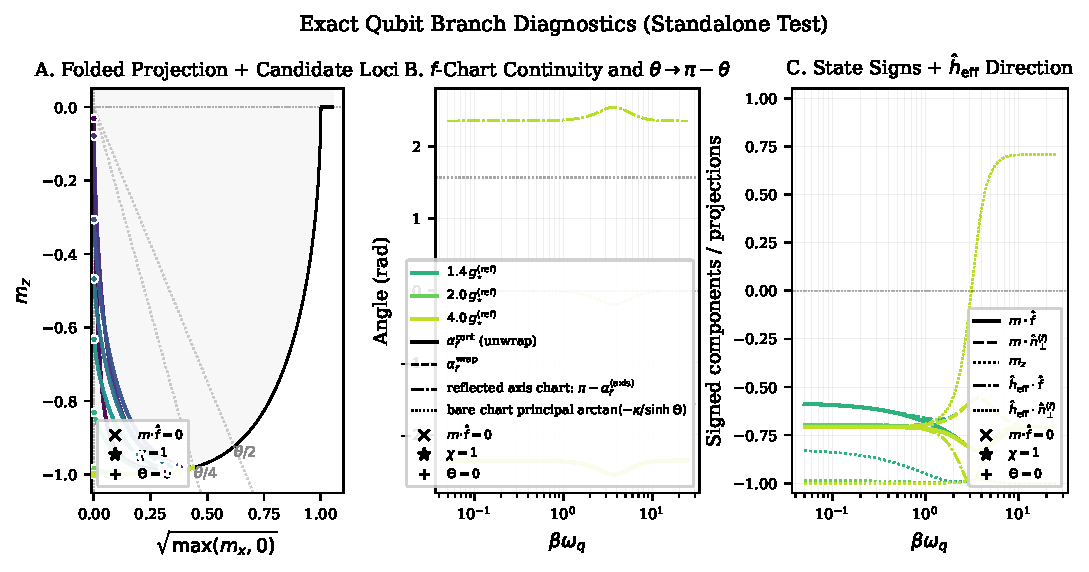
\includegraphics[width=\linewidth]{../figures/hmf_branch_flip_test}
    \caption{
        Standalone branch-diagnostics overview (exact qubit model). Panel A
        reproduces the folded-projection geometry relevant to
        Fig.~\ref{fig:bloch_disk_portrait}(b), while Panels B--C compare
        principal-chart and continuity-corrected angular descriptions together
        with signed component projections. The purpose of this figure is to
        expose how a folded/projection chart can make a continuous precession
        appear as a reflection, and to separate crossover markers ($\chi=1$)
        from genuine angle-chart singular loci.
    }
    \label{fig:branch_codex_diag_overview}
\end{figure*}

\begin{figure*}[t]
    \centering
    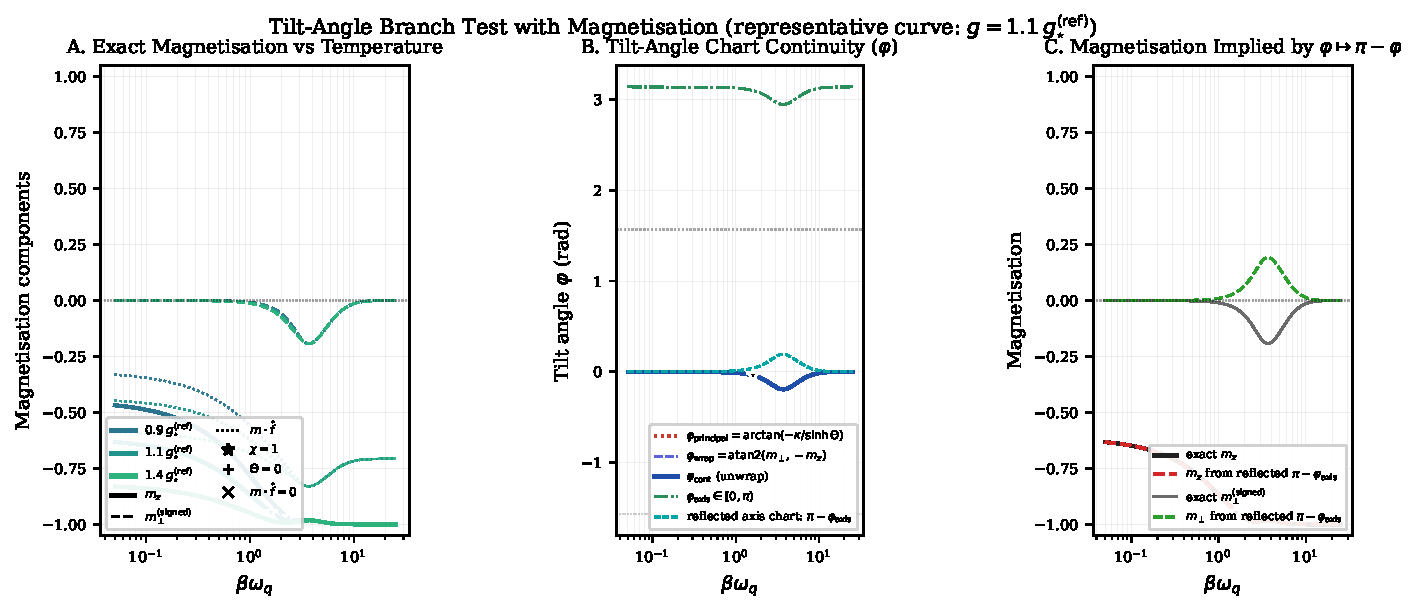
\includegraphics[width=\linewidth]{../figures/hmf_tilt_magnetisation_branch_test}
    \caption{
        Standalone tilt-angle and magnetisation test for the
        branch-continuation argument. The plotted magnetisation components make
        explicit that the physical Bloch vector remains continuous, while the
        principal tilt angle can jump by a chart branch crossing. Comparing the
        principal angle, continuity-corrected angle, and the reflected
        axis-chart continuation demonstrates the appendix claim: the visually
        apparent reflection in the folded representation is resolved by a
        continuous angular continuation toward alignment with $\hat{\mathbf f}$,
        not by a physical bounce at the principal-chart image $\pi-\alpha_f$.
    }
    \label{fig:branch_codex_diag_tilt_mag}
\end{figure*}

\begin{figure*}[t]
    \centering
    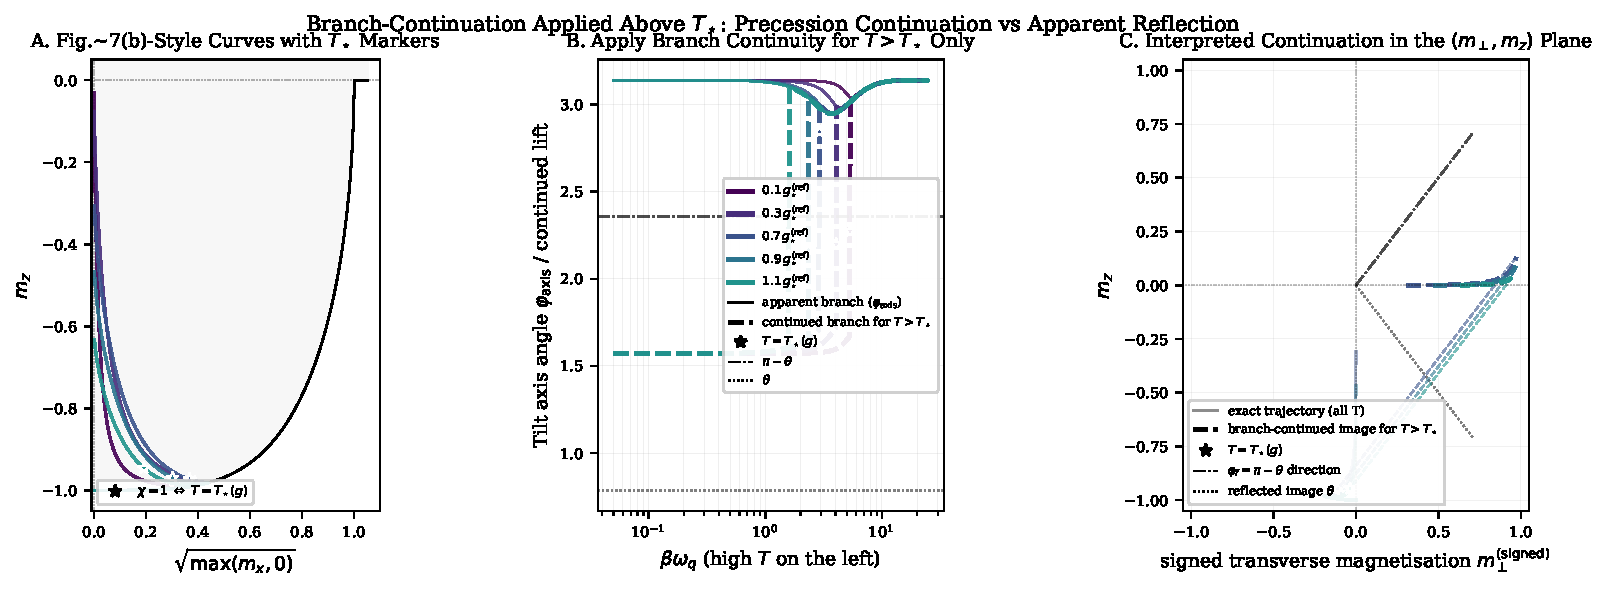
\includegraphics[width=\linewidth]{../figures/hmf_tstar_branch_continuation_demo}
    \caption{
        Explicit branch-continuation construction applied to the Fig.~7(b)-style
        curves. The crossover marker $T=T_\star(g)$ (equivalently $\chi=1$)
        partitions each trajectory, and the plotted overlay applies the
        director/axis continuity rule only on the $T>T_\star$ segment
        (high-temperature side) so that the tilt-angle branch is continued as a
        precession rather than read as a reflection at the principal-chart
        image. Panel B shows the piecewise continuation in the tilt-axis angle
        chart relative to the reference directions $\theta$ and $\pi-\theta$;
        Panel C maps that continuation back into the $(m_\perp,m_z)$ plane as
        an interpretive branch-resolved overlay. This figure is the direct
        visualization of the appendix claim that the apparent reflection can be
        re-read as a continuity-corrected approach toward the interaction-axis
        sector.
    }
    \label{fig:branch_codex_tstar_cont_demo}
\end{figure*}

\begin{figure*}[t]
    \centering
    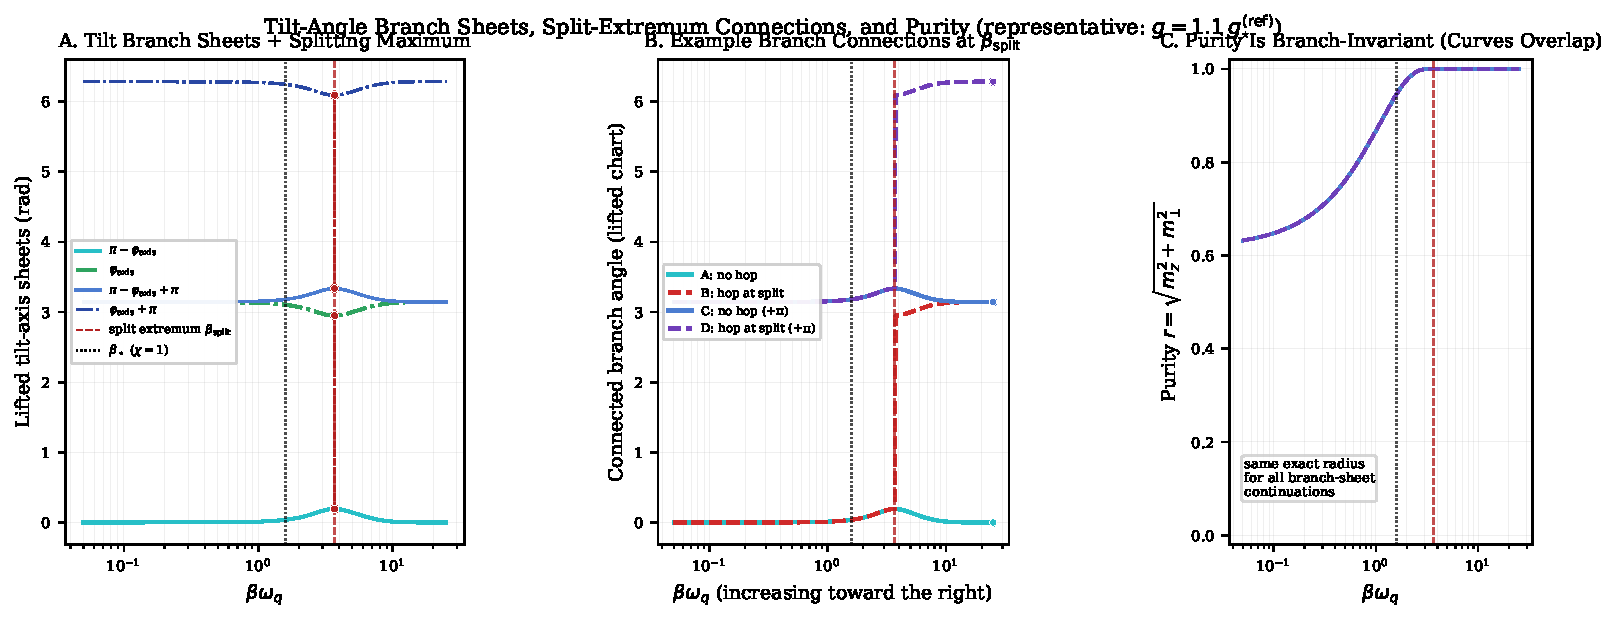
\includegraphics[width=\linewidth]{../figures/hmf_tilt_branch_sheet_purity_demo}
    \caption{
        Tilt-angle branch-sheet construction (representative coupling) showing
        how different lifted branch connections can be spliced at the splitting
        extremum of the visible branch separation, and how those distinct branch
        continuations flow to different asymptotic angle values as
        $\beta\rightarrow\infty$. Panel A displays the lifted tilt-axis sheets
        and marks both the crossover point $\beta_\star$ ($\chi=1$) and the
        splitting extremum $\beta_{\rm split}$. Panel B shows example branch
        connections obtained by switching sheets at $\beta_{\rm split}$.
        Panel C plots the corresponding purities and shows that they are
        branch-invariant: all branch-sheet continuations share the same exact
        radius $r=\sqrt{m_z^2+m_\perp^2}=\tanh\chi$. This is the visual
        ``seal'' of the appendix argument that the branch multiplicity is an
        angular-sheet/continuation structure on top of a single purity
        crossover.
    }
    \label{fig:branch_codex_tilt_sheet_purity}
\end{figure*}

\begin{figure*}[t]
    \centering
    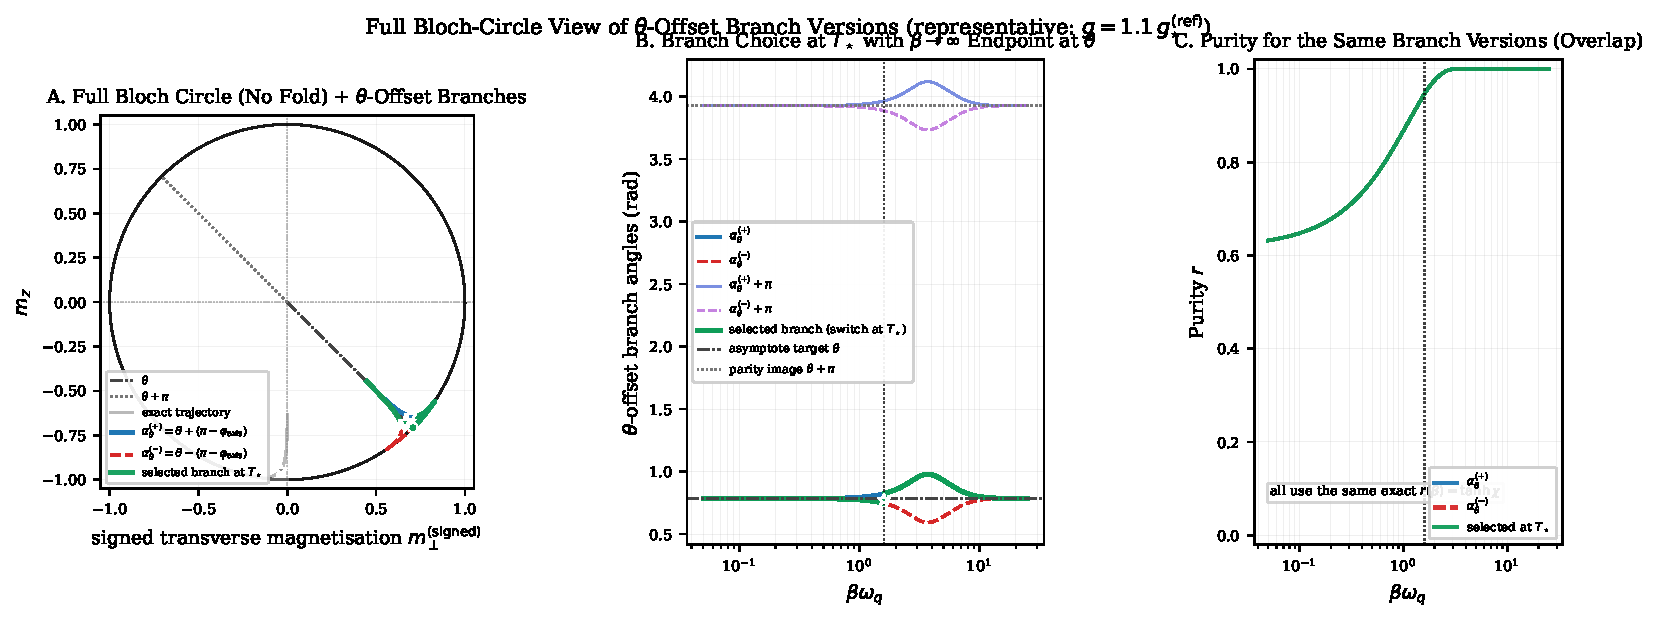
\includegraphics[width=\linewidth]{../figures/hmf_full_bloch_theta_branch_demo}
    \caption{
        Full Bloch-circle (unfolded) visualization of $\theta$-offset branch
        versions for a representative coupling. Unlike the folded
        $\sqrt{m_x}$ portrait, Panel A shows the full coupling-plane circle and
        overlays branch versions constructed so that one selected branch (green)
        switches at $T_\star$ and approaches the original angle $\theta$ as
        $\beta\to\infty$. Panel B shows the corresponding $\theta$-offset angle
        versions and the explicit branch choice at $T_\star$, together with the
        asymptote targets $\theta$ and $\theta+\pi$. Panel C confirms that all
        these branch versions share the same exact purity $r(\beta)=\tanh\chi$.
        This figure is the appendix's direct answer to the ``full Bloch circle''
        branch-continuation question: the branch choice changes the angular
        sheet/endpoint interpretation while leaving the exact purity unchanged.
    }
    \label{fig:branch_codex_full_bloch_theta_demo}
\end{figure*}
